
% Default to the notebook output style

    


% Inherit from the specified cell style.




    
\documentclass[11pt]{article}

    
    
    \usepackage[T1]{fontenc}
    % Nicer default font (+ math font) than Computer Modern for most use cases
    \usepackage{mathpazo}

    % Basic figure setup, for now with no caption control since it's done
    % automatically by Pandoc (which extracts ![](path) syntax from Markdown).
    \usepackage{graphicx}
    % We will generate all images so they have a width \maxwidth. This means
    % that they will get their normal width if they fit onto the page, but
    % are scaled down if they would overflow the margins.
    \makeatletter
    \def\maxwidth{\ifdim\Gin@nat@width>\linewidth\linewidth
    \else\Gin@nat@width\fi}
    \makeatother
    \let\Oldincludegraphics\includegraphics
    % Set max figure width to be 80% of text width, for now hardcoded.
    \renewcommand{\includegraphics}[1]{\Oldincludegraphics[width=.8\maxwidth]{#1}}
    % Ensure that by default, figures have no caption (until we provide a
    % proper Figure object with a Caption API and a way to capture that
    % in the conversion process - todo).
    \usepackage{caption}
    \DeclareCaptionLabelFormat{nolabel}{}
    \captionsetup{labelformat=nolabel}

    \usepackage{adjustbox} % Used to constrain images to a maximum size 
    \usepackage{xcolor} % Allow colors to be defined
    \usepackage{enumerate} % Needed for markdown enumerations to work
    \usepackage{geometry} % Used to adjust the document margins
    \usepackage{amsmath} % Equations
    \usepackage{amssymb} % Equations
    \usepackage{textcomp} % defines textquotesingle
    % Hack from http://tex.stackexchange.com/a/47451/13684:
    \AtBeginDocument{%
        \def\PYZsq{\textquotesingle}% Upright quotes in Pygmentized code
    }
    \usepackage{upquote} % Upright quotes for verbatim code
    \usepackage{eurosym} % defines \euro
    \usepackage[mathletters]{ucs} % Extended unicode (utf-8) support
    \usepackage[utf8x]{inputenc} % Allow utf-8 characters in the tex document
    \usepackage{fancyvrb} % verbatim replacement that allows latex
    \usepackage{grffile} % extends the file name processing of package graphics 
                         % to support a larger range 
    % The hyperref package gives us a pdf with properly built
    % internal navigation ('pdf bookmarks' for the table of contents,
    % internal cross-reference links, web links for URLs, etc.)
    \usepackage{hyperref}
    \usepackage{longtable} % longtable support required by pandoc >1.10
    \usepackage{booktabs}  % table support for pandoc > 1.12.2
    \usepackage[inline]{enumitem} % IRkernel/repr support (it uses the enumerate* environment)
    \usepackage[normalem]{ulem} % ulem is needed to support strikethroughs (\sout)
                                % normalem makes italics be italics, not underlines
    

    
    
    % Colors for the hyperref package
    \definecolor{urlcolor}{rgb}{0,.145,.698}
    \definecolor{linkcolor}{rgb}{.71,0.21,0.01}
    \definecolor{citecolor}{rgb}{.12,.54,.11}

    % ANSI colors
    \definecolor{ansi-black}{HTML}{3E424D}
    \definecolor{ansi-black-intense}{HTML}{282C36}
    \definecolor{ansi-red}{HTML}{E75C58}
    \definecolor{ansi-red-intense}{HTML}{B22B31}
    \definecolor{ansi-green}{HTML}{00A250}
    \definecolor{ansi-green-intense}{HTML}{007427}
    \definecolor{ansi-yellow}{HTML}{DDB62B}
    \definecolor{ansi-yellow-intense}{HTML}{B27D12}
    \definecolor{ansi-blue}{HTML}{208FFB}
    \definecolor{ansi-blue-intense}{HTML}{0065CA}
    \definecolor{ansi-magenta}{HTML}{D160C4}
    \definecolor{ansi-magenta-intense}{HTML}{A03196}
    \definecolor{ansi-cyan}{HTML}{60C6C8}
    \definecolor{ansi-cyan-intense}{HTML}{258F8F}
    \definecolor{ansi-white}{HTML}{C5C1B4}
    \definecolor{ansi-white-intense}{HTML}{A1A6B2}

    % commands and environments needed by pandoc snippets
    % extracted from the output of `pandoc -s`
    \providecommand{\tightlist}{%
      \setlength{\itemsep}{0pt}\setlength{\parskip}{0pt}}
    \DefineVerbatimEnvironment{Highlighting}{Verbatim}{commandchars=\\\{\}}
    % Add ',fontsize=\small' for more characters per line
    \newenvironment{Shaded}{}{}
    \newcommand{\KeywordTok}[1]{\textcolor[rgb]{0.00,0.44,0.13}{\textbf{{#1}}}}
    \newcommand{\DataTypeTok}[1]{\textcolor[rgb]{0.56,0.13,0.00}{{#1}}}
    \newcommand{\DecValTok}[1]{\textcolor[rgb]{0.25,0.63,0.44}{{#1}}}
    \newcommand{\BaseNTok}[1]{\textcolor[rgb]{0.25,0.63,0.44}{{#1}}}
    \newcommand{\FloatTok}[1]{\textcolor[rgb]{0.25,0.63,0.44}{{#1}}}
    \newcommand{\CharTok}[1]{\textcolor[rgb]{0.25,0.44,0.63}{{#1}}}
    \newcommand{\StringTok}[1]{\textcolor[rgb]{0.25,0.44,0.63}{{#1}}}
    \newcommand{\CommentTok}[1]{\textcolor[rgb]{0.38,0.63,0.69}{\textit{{#1}}}}
    \newcommand{\OtherTok}[1]{\textcolor[rgb]{0.00,0.44,0.13}{{#1}}}
    \newcommand{\AlertTok}[1]{\textcolor[rgb]{1.00,0.00,0.00}{\textbf{{#1}}}}
    \newcommand{\FunctionTok}[1]{\textcolor[rgb]{0.02,0.16,0.49}{{#1}}}
    \newcommand{\RegionMarkerTok}[1]{{#1}}
    \newcommand{\ErrorTok}[1]{\textcolor[rgb]{1.00,0.00,0.00}{\textbf{{#1}}}}
    \newcommand{\NormalTok}[1]{{#1}}
    
    % Additional commands for more recent versions of Pandoc
    \newcommand{\ConstantTok}[1]{\textcolor[rgb]{0.53,0.00,0.00}{{#1}}}
    \newcommand{\SpecialCharTok}[1]{\textcolor[rgb]{0.25,0.44,0.63}{{#1}}}
    \newcommand{\VerbatimStringTok}[1]{\textcolor[rgb]{0.25,0.44,0.63}{{#1}}}
    \newcommand{\SpecialStringTok}[1]{\textcolor[rgb]{0.73,0.40,0.53}{{#1}}}
    \newcommand{\ImportTok}[1]{{#1}}
    \newcommand{\DocumentationTok}[1]{\textcolor[rgb]{0.73,0.13,0.13}{\textit{{#1}}}}
    \newcommand{\AnnotationTok}[1]{\textcolor[rgb]{0.38,0.63,0.69}{\textbf{\textit{{#1}}}}}
    \newcommand{\CommentVarTok}[1]{\textcolor[rgb]{0.38,0.63,0.69}{\textbf{\textit{{#1}}}}}
    \newcommand{\VariableTok}[1]{\textcolor[rgb]{0.10,0.09,0.49}{{#1}}}
    \newcommand{\ControlFlowTok}[1]{\textcolor[rgb]{0.00,0.44,0.13}{\textbf{{#1}}}}
    \newcommand{\OperatorTok}[1]{\textcolor[rgb]{0.40,0.40,0.40}{{#1}}}
    \newcommand{\BuiltInTok}[1]{{#1}}
    \newcommand{\ExtensionTok}[1]{{#1}}
    \newcommand{\PreprocessorTok}[1]{\textcolor[rgb]{0.74,0.48,0.00}{{#1}}}
    \newcommand{\AttributeTok}[1]{\textcolor[rgb]{0.49,0.56,0.16}{{#1}}}
    \newcommand{\InformationTok}[1]{\textcolor[rgb]{0.38,0.63,0.69}{\textbf{\textit{{#1}}}}}
    \newcommand{\WarningTok}[1]{\textcolor[rgb]{0.38,0.63,0.69}{\textbf{\textit{{#1}}}}}
    
    
    % Define a nice break command that doesn't care if a line doesn't already
    % exist.
    \def\br{\hspace*{\fill} \\* }
    % Math Jax compatability definitions
    \def\gt{>}
    \def\lt{<}
    % Document parameters
    \title{Intro to SQL}
    
    
    

    % Pygments definitions
    
\makeatletter
\def\PY@reset{\let\PY@it=\relax \let\PY@bf=\relax%
    \let\PY@ul=\relax \let\PY@tc=\relax%
    \let\PY@bc=\relax \let\PY@ff=\relax}
\def\PY@tok#1{\csname PY@tok@#1\endcsname}
\def\PY@toks#1+{\ifx\relax#1\empty\else%
    \PY@tok{#1}\expandafter\PY@toks\fi}
\def\PY@do#1{\PY@bc{\PY@tc{\PY@ul{%
    \PY@it{\PY@bf{\PY@ff{#1}}}}}}}
\def\PY#1#2{\PY@reset\PY@toks#1+\relax+\PY@do{#2}}

\expandafter\def\csname PY@tok@w\endcsname{\def\PY@tc##1{\textcolor[rgb]{0.73,0.73,0.73}{##1}}}
\expandafter\def\csname PY@tok@c\endcsname{\let\PY@it=\textit\def\PY@tc##1{\textcolor[rgb]{0.25,0.50,0.50}{##1}}}
\expandafter\def\csname PY@tok@cp\endcsname{\def\PY@tc##1{\textcolor[rgb]{0.74,0.48,0.00}{##1}}}
\expandafter\def\csname PY@tok@k\endcsname{\let\PY@bf=\textbf\def\PY@tc##1{\textcolor[rgb]{0.00,0.50,0.00}{##1}}}
\expandafter\def\csname PY@tok@kp\endcsname{\def\PY@tc##1{\textcolor[rgb]{0.00,0.50,0.00}{##1}}}
\expandafter\def\csname PY@tok@kt\endcsname{\def\PY@tc##1{\textcolor[rgb]{0.69,0.00,0.25}{##1}}}
\expandafter\def\csname PY@tok@o\endcsname{\def\PY@tc##1{\textcolor[rgb]{0.40,0.40,0.40}{##1}}}
\expandafter\def\csname PY@tok@ow\endcsname{\let\PY@bf=\textbf\def\PY@tc##1{\textcolor[rgb]{0.67,0.13,1.00}{##1}}}
\expandafter\def\csname PY@tok@nb\endcsname{\def\PY@tc##1{\textcolor[rgb]{0.00,0.50,0.00}{##1}}}
\expandafter\def\csname PY@tok@nf\endcsname{\def\PY@tc##1{\textcolor[rgb]{0.00,0.00,1.00}{##1}}}
\expandafter\def\csname PY@tok@nc\endcsname{\let\PY@bf=\textbf\def\PY@tc##1{\textcolor[rgb]{0.00,0.00,1.00}{##1}}}
\expandafter\def\csname PY@tok@nn\endcsname{\let\PY@bf=\textbf\def\PY@tc##1{\textcolor[rgb]{0.00,0.00,1.00}{##1}}}
\expandafter\def\csname PY@tok@ne\endcsname{\let\PY@bf=\textbf\def\PY@tc##1{\textcolor[rgb]{0.82,0.25,0.23}{##1}}}
\expandafter\def\csname PY@tok@nv\endcsname{\def\PY@tc##1{\textcolor[rgb]{0.10,0.09,0.49}{##1}}}
\expandafter\def\csname PY@tok@no\endcsname{\def\PY@tc##1{\textcolor[rgb]{0.53,0.00,0.00}{##1}}}
\expandafter\def\csname PY@tok@nl\endcsname{\def\PY@tc##1{\textcolor[rgb]{0.63,0.63,0.00}{##1}}}
\expandafter\def\csname PY@tok@ni\endcsname{\let\PY@bf=\textbf\def\PY@tc##1{\textcolor[rgb]{0.60,0.60,0.60}{##1}}}
\expandafter\def\csname PY@tok@na\endcsname{\def\PY@tc##1{\textcolor[rgb]{0.49,0.56,0.16}{##1}}}
\expandafter\def\csname PY@tok@nt\endcsname{\let\PY@bf=\textbf\def\PY@tc##1{\textcolor[rgb]{0.00,0.50,0.00}{##1}}}
\expandafter\def\csname PY@tok@nd\endcsname{\def\PY@tc##1{\textcolor[rgb]{0.67,0.13,1.00}{##1}}}
\expandafter\def\csname PY@tok@s\endcsname{\def\PY@tc##1{\textcolor[rgb]{0.73,0.13,0.13}{##1}}}
\expandafter\def\csname PY@tok@sd\endcsname{\let\PY@it=\textit\def\PY@tc##1{\textcolor[rgb]{0.73,0.13,0.13}{##1}}}
\expandafter\def\csname PY@tok@si\endcsname{\let\PY@bf=\textbf\def\PY@tc##1{\textcolor[rgb]{0.73,0.40,0.53}{##1}}}
\expandafter\def\csname PY@tok@se\endcsname{\let\PY@bf=\textbf\def\PY@tc##1{\textcolor[rgb]{0.73,0.40,0.13}{##1}}}
\expandafter\def\csname PY@tok@sr\endcsname{\def\PY@tc##1{\textcolor[rgb]{0.73,0.40,0.53}{##1}}}
\expandafter\def\csname PY@tok@ss\endcsname{\def\PY@tc##1{\textcolor[rgb]{0.10,0.09,0.49}{##1}}}
\expandafter\def\csname PY@tok@sx\endcsname{\def\PY@tc##1{\textcolor[rgb]{0.00,0.50,0.00}{##1}}}
\expandafter\def\csname PY@tok@m\endcsname{\def\PY@tc##1{\textcolor[rgb]{0.40,0.40,0.40}{##1}}}
\expandafter\def\csname PY@tok@gh\endcsname{\let\PY@bf=\textbf\def\PY@tc##1{\textcolor[rgb]{0.00,0.00,0.50}{##1}}}
\expandafter\def\csname PY@tok@gu\endcsname{\let\PY@bf=\textbf\def\PY@tc##1{\textcolor[rgb]{0.50,0.00,0.50}{##1}}}
\expandafter\def\csname PY@tok@gd\endcsname{\def\PY@tc##1{\textcolor[rgb]{0.63,0.00,0.00}{##1}}}
\expandafter\def\csname PY@tok@gi\endcsname{\def\PY@tc##1{\textcolor[rgb]{0.00,0.63,0.00}{##1}}}
\expandafter\def\csname PY@tok@gr\endcsname{\def\PY@tc##1{\textcolor[rgb]{1.00,0.00,0.00}{##1}}}
\expandafter\def\csname PY@tok@ge\endcsname{\let\PY@it=\textit}
\expandafter\def\csname PY@tok@gs\endcsname{\let\PY@bf=\textbf}
\expandafter\def\csname PY@tok@gp\endcsname{\let\PY@bf=\textbf\def\PY@tc##1{\textcolor[rgb]{0.00,0.00,0.50}{##1}}}
\expandafter\def\csname PY@tok@go\endcsname{\def\PY@tc##1{\textcolor[rgb]{0.53,0.53,0.53}{##1}}}
\expandafter\def\csname PY@tok@gt\endcsname{\def\PY@tc##1{\textcolor[rgb]{0.00,0.27,0.87}{##1}}}
\expandafter\def\csname PY@tok@err\endcsname{\def\PY@bc##1{\setlength{\fboxsep}{0pt}\fcolorbox[rgb]{1.00,0.00,0.00}{1,1,1}{\strut ##1}}}
\expandafter\def\csname PY@tok@kc\endcsname{\let\PY@bf=\textbf\def\PY@tc##1{\textcolor[rgb]{0.00,0.50,0.00}{##1}}}
\expandafter\def\csname PY@tok@kd\endcsname{\let\PY@bf=\textbf\def\PY@tc##1{\textcolor[rgb]{0.00,0.50,0.00}{##1}}}
\expandafter\def\csname PY@tok@kn\endcsname{\let\PY@bf=\textbf\def\PY@tc##1{\textcolor[rgb]{0.00,0.50,0.00}{##1}}}
\expandafter\def\csname PY@tok@kr\endcsname{\let\PY@bf=\textbf\def\PY@tc##1{\textcolor[rgb]{0.00,0.50,0.00}{##1}}}
\expandafter\def\csname PY@tok@bp\endcsname{\def\PY@tc##1{\textcolor[rgb]{0.00,0.50,0.00}{##1}}}
\expandafter\def\csname PY@tok@fm\endcsname{\def\PY@tc##1{\textcolor[rgb]{0.00,0.00,1.00}{##1}}}
\expandafter\def\csname PY@tok@vc\endcsname{\def\PY@tc##1{\textcolor[rgb]{0.10,0.09,0.49}{##1}}}
\expandafter\def\csname PY@tok@vg\endcsname{\def\PY@tc##1{\textcolor[rgb]{0.10,0.09,0.49}{##1}}}
\expandafter\def\csname PY@tok@vi\endcsname{\def\PY@tc##1{\textcolor[rgb]{0.10,0.09,0.49}{##1}}}
\expandafter\def\csname PY@tok@vm\endcsname{\def\PY@tc##1{\textcolor[rgb]{0.10,0.09,0.49}{##1}}}
\expandafter\def\csname PY@tok@sa\endcsname{\def\PY@tc##1{\textcolor[rgb]{0.73,0.13,0.13}{##1}}}
\expandafter\def\csname PY@tok@sb\endcsname{\def\PY@tc##1{\textcolor[rgb]{0.73,0.13,0.13}{##1}}}
\expandafter\def\csname PY@tok@sc\endcsname{\def\PY@tc##1{\textcolor[rgb]{0.73,0.13,0.13}{##1}}}
\expandafter\def\csname PY@tok@dl\endcsname{\def\PY@tc##1{\textcolor[rgb]{0.73,0.13,0.13}{##1}}}
\expandafter\def\csname PY@tok@s2\endcsname{\def\PY@tc##1{\textcolor[rgb]{0.73,0.13,0.13}{##1}}}
\expandafter\def\csname PY@tok@sh\endcsname{\def\PY@tc##1{\textcolor[rgb]{0.73,0.13,0.13}{##1}}}
\expandafter\def\csname PY@tok@s1\endcsname{\def\PY@tc##1{\textcolor[rgb]{0.73,0.13,0.13}{##1}}}
\expandafter\def\csname PY@tok@mb\endcsname{\def\PY@tc##1{\textcolor[rgb]{0.40,0.40,0.40}{##1}}}
\expandafter\def\csname PY@tok@mf\endcsname{\def\PY@tc##1{\textcolor[rgb]{0.40,0.40,0.40}{##1}}}
\expandafter\def\csname PY@tok@mh\endcsname{\def\PY@tc##1{\textcolor[rgb]{0.40,0.40,0.40}{##1}}}
\expandafter\def\csname PY@tok@mi\endcsname{\def\PY@tc##1{\textcolor[rgb]{0.40,0.40,0.40}{##1}}}
\expandafter\def\csname PY@tok@il\endcsname{\def\PY@tc##1{\textcolor[rgb]{0.40,0.40,0.40}{##1}}}
\expandafter\def\csname PY@tok@mo\endcsname{\def\PY@tc##1{\textcolor[rgb]{0.40,0.40,0.40}{##1}}}
\expandafter\def\csname PY@tok@ch\endcsname{\let\PY@it=\textit\def\PY@tc##1{\textcolor[rgb]{0.25,0.50,0.50}{##1}}}
\expandafter\def\csname PY@tok@cm\endcsname{\let\PY@it=\textit\def\PY@tc##1{\textcolor[rgb]{0.25,0.50,0.50}{##1}}}
\expandafter\def\csname PY@tok@cpf\endcsname{\let\PY@it=\textit\def\PY@tc##1{\textcolor[rgb]{0.25,0.50,0.50}{##1}}}
\expandafter\def\csname PY@tok@c1\endcsname{\let\PY@it=\textit\def\PY@tc##1{\textcolor[rgb]{0.25,0.50,0.50}{##1}}}
\expandafter\def\csname PY@tok@cs\endcsname{\let\PY@it=\textit\def\PY@tc##1{\textcolor[rgb]{0.25,0.50,0.50}{##1}}}

\def\PYZbs{\char`\\}
\def\PYZus{\char`\_}
\def\PYZob{\char`\{}
\def\PYZcb{\char`\}}
\def\PYZca{\char`\^}
\def\PYZam{\char`\&}
\def\PYZlt{\char`\<}
\def\PYZgt{\char`\>}
\def\PYZsh{\char`\#}
\def\PYZpc{\char`\%}
\def\PYZdl{\char`\$}
\def\PYZhy{\char`\-}
\def\PYZsq{\char`\'}
\def\PYZdq{\char`\"}
\def\PYZti{\char`\~}
% for compatibility with earlier versions
\def\PYZat{@}
\def\PYZlb{[}
\def\PYZrb{]}
\makeatother


    % Exact colors from NB
    \definecolor{incolor}{rgb}{0.0, 0.0, 0.5}
    \definecolor{outcolor}{rgb}{0.545, 0.0, 0.0}



    
    % Prevent overflowing lines due to hard-to-break entities
    \sloppy 
    % Setup hyperref package
    \hypersetup{
      breaklinks=true,  % so long urls are correctly broken across lines
      colorlinks=true,
      urlcolor=urlcolor,
      linkcolor=linkcolor,
      citecolor=citecolor,
      }
    % Slightly bigger margins than the latex defaults
    
    \geometry{verbose,tmargin=1in,bmargin=1in,lmargin=1in,rmargin=1in}
    
    

    \begin{document}
    
    
    \maketitle
    
    

    
    \hypertarget{factbook-database-from-cia}{%
\subsubsection{Factbook Database from
CIA}\label{factbook-database-from-cia}}

https://github.com/factbook/factbook.sql

\begin{verbatim}
CREATE TABLE "facts" (
  "id" INTEGER PRIMARY KEY AUTOINCREMENT NOT NULL,
  "code" varchar(255) NOT NULL,
  "name" varchar(255) NOT NULL,
  
  ---------------------------------------
  -- Geography
  "area"       integer,
  "area_land"  integer,
  "area_water" integer,
  
  ----------------------------------------
  -- People and Society
  "population"        integer,
  "population_growth" float,
  "birth_rate"        float,
  "death_rate"        float,
  "migration_rate"    float,
  
  --------------------------------
  -- Timestamp
  "created_at" datetime,
  "updated_at" datetime
)
\end{verbatim}

    \hypertarget{select-where}{%
\subsubsection{SELECT / WHERE}\label{select-where}}

\begin{verbatim}
SELECT column_name(s)
FROM table_name
WHERE condition AND|OR condition
\end{verbatim}

    \begin{Verbatim}[commandchars=\\\{\}]
{\color{incolor}In [{\color{incolor}1}]:} \PY{k+kn}{import} \PY{n+nn}{sqlite3}
        \PY{k+kn}{import} \PY{n+nn}{pandas} \PY{k}{as} \PY{n+nn}{pd}
        
        \PY{n}{conn} \PY{o}{=} \PY{n}{sqlite3}\PY{o}{.}\PY{n}{connect}\PY{p}{(}\PY{l+s+s2}{\PYZdq{}}\PY{l+s+s2}{factbook.db}\PY{l+s+s2}{\PYZdq{}}\PY{p}{)}
        \PY{n}{facts} \PY{o}{=} \PY{n}{pd}\PY{o}{.}\PY{n}{read\PYZus{}sql\PYZus{}query}\PY{p}{(}\PY{l+s+s2}{\PYZdq{}}\PY{l+s+s2}{SELECT * FROM facts;}\PY{l+s+s2}{\PYZdq{}}\PY{p}{,}\PY{n}{conn}\PY{p}{)}
        \PY{n}{facts}\PY{o}{.}\PY{n}{head}\PY{p}{(}\PY{l+m+mi}{5}\PY{p}{)}
\end{Verbatim}


\begin{Verbatim}[commandchars=\\\{\}]
{\color{outcolor}Out[{\color{outcolor}1}]:}    id code         name       area  area\_land  area\_water  population  \textbackslash{}
        0   1   af  Afghanistan   652230.0   652230.0         0.0  32564342.0   
        1   2   al      Albania    28748.0    27398.0      1350.0   3029278.0   
        2   3   ag      Algeria  2381741.0  2381741.0         0.0  39542166.0   
        3   4   an      Andorra      468.0      468.0         0.0     85580.0   
        4   5   ao       Angola  1246700.0  1246700.0         0.0  19625353.0   
        
           population\_growth  birth\_rate  death\_rate  migration\_rate  \textbackslash{}
        0               2.32       38.57       13.89            1.51   
        1               0.30       12.92        6.58            3.30   
        2               1.84       23.67        4.31            0.92   
        3               0.12        8.13        6.96            0.00   
        4               2.78       38.78       11.49            0.46   
        
                           created\_at                  updated\_at  
        0  2015-11-01 13:19:49.461734  2015-11-01 13:19:49.461734  
        1  2015-11-01 13:19:54.431082  2015-11-01 13:19:54.431082  
        2  2015-11-01 13:19:59.961286  2015-11-01 13:19:59.961286  
        3  2015-11-01 13:20:03.659945  2015-11-01 13:20:03.659945  
        4  2015-11-01 13:20:08.625072  2015-11-01 13:20:08.625072  
\end{Verbatim}
            
    \hypertarget{ux3b1ux3c1ux3b9ux3b8ux3bcux3ccux3c2-ux3b3ux3c1ux3b1ux3bcux3bcux3ceux3bd}{%
\subsubsection{Αριθμός
γραμμών}\label{ux3b1ux3c1ux3b9ux3b8ux3bcux3ccux3c2-ux3b3ux3c1ux3b1ux3bcux3bcux3ceux3bd}}

    \begin{Verbatim}[commandchars=\\\{\}]
{\color{incolor}In [{\color{incolor}2}]:} \PY{n}{facts}\PY{o}{.}\PY{n}{shape}
\end{Verbatim}


\begin{Verbatim}[commandchars=\\\{\}]
{\color{outcolor}Out[{\color{outcolor}2}]:} (261, 13)
\end{Verbatim}
            
    \hypertarget{ux3b5ux3c1ux3ceux3c4ux3b7ux3bcux3b1-ux3bcux3b5-ux3c3ux3c5ux3b3ux3baux3b5ux3baux3c1ux3b9ux3bcux3adux3bdux3b5ux3c2-ux3c3ux3c4ux3aeux3bbux3b5ux3c2}{%
\subsubsection{Ερώτημα με συγκεκριμένες
στήλες}\label{ux3b5ux3c1ux3ceux3c4ux3b7ux3bcux3b1-ux3bcux3b5-ux3c3ux3c5ux3b3ux3baux3b5ux3baux3c1ux3b9ux3bcux3adux3bdux3b5ux3c2-ux3c3ux3c4ux3aeux3bbux3b5ux3c2}}

\begin{verbatim}
SELECT name, population 
FROM facts
\end{verbatim}

    \begin{Verbatim}[commandchars=\\\{\}]
{\color{incolor}In [{\color{incolor}3}]:} \PY{n}{facts} \PY{o}{=} \PY{n}{pd}\PY{o}{.}\PY{n}{read\PYZus{}sql\PYZus{}query}\PY{p}{(}\PY{l+s+s2}{\PYZdq{}}\PY{l+s+s2}{SELECT name, population FROM facts;}\PY{l+s+s2}{\PYZdq{}}\PY{p}{,}\PY{n}{conn}\PY{p}{)}
        \PY{n}{facts}\PY{o}{.}\PY{n}{head}\PY{p}{(}\PY{l+m+mi}{5}\PY{p}{)}
\end{Verbatim}


\begin{Verbatim}[commandchars=\\\{\}]
{\color{outcolor}Out[{\color{outcolor}3}]:}           name  population
        0  Afghanistan  32564342.0
        1      Albania   3029278.0
        2      Algeria  39542166.0
        3      Andorra     85580.0
        4       Angola  19625353.0
\end{Verbatim}
            
    \hypertarget{ux3ae-ux3bcux3b5-ux3c3ux3c5ux3b3ux3baux3b5ux3baux3c1ux3b9ux3bcux3adux3bdux3b5ux3c2-ux3b3ux3c1ux3b1ux3bcux3bcux3adux3c2}{%
\subsubsection{Ή με συγκεκριμένες
γραμμές}\label{ux3ae-ux3bcux3b5-ux3c3ux3c5ux3b3ux3baux3b5ux3baux3c1ux3b9ux3bcux3adux3bdux3b5ux3c2-ux3b3ux3c1ux3b1ux3bcux3bcux3adux3c2}}

    \begin{verbatim}
SELECT name, population 
FROM facts 
WHERE population > 50000000
\end{verbatim}

    \begin{Verbatim}[commandchars=\\\{\}]
{\color{incolor}In [{\color{incolor}4}]:} \PY{n}{pd}\PY{o}{.}\PY{n}{read\PYZus{}sql\PYZus{}query}\PY{p}{(}\PY{l+s+s2}{\PYZdq{}}\PY{l+s+s2}{SELECT name, population FROM facts WHERE population \PYZgt{} 50000000;}\PY{l+s+s2}{\PYZdq{}}\PY{p}{,}\PY{n}{conn}\PY{p}{)}
\end{Verbatim}


\begin{Verbatim}[commandchars=\\\{\}]
{\color{outcolor}Out[{\color{outcolor}4}]:}                                  name  population
        0                          Bangladesh   168957745
        1                              Brazil   204259812
        2                               Burma    56320206
        3                               China  1367485388
        4   Congo, Democratic Republic of the    79375136
        5                               Egypt    88487396
        6                            Ethiopia    99465819
        7                              France    66553766
        8                             Germany    80854408
        9                               India  1251695584
        10                          Indonesia   255993674
        11                               Iran    81824270
        12                              Italy    61855120
        13                              Japan   126919659
        14                             Mexico   121736809
        15                            Nigeria   181562056
        16                           Pakistan   199085847
        17                        Philippines   100998376
        18                             Russia   142423773
        19                       South Africa    53675563
        20                           Tanzania    51045882
        21                           Thailand    67976405
        22                             Turkey    79414269
        23                     United Kingdom    64088222
        24                      United States   321368864
        25                            Vietnam    94348835
        26                     European Union   513949445
        27                              World  7256490011
\end{Verbatim}
            
    \begin{verbatim}
SELECT name, population 
FROM facts 
WHERE population BETWEEN 10000000 AND 20000000
\end{verbatim}

    \begin{Verbatim}[commandchars=\\\{\}]
{\color{incolor}In [{\color{incolor}5}]:} \PY{n}{pd}\PY{o}{.}\PY{n}{read\PYZus{}sql\PYZus{}query}\PY{p}{(}\PY{l+s+s2}{\PYZdq{}}\PY{l+s+s2}{SELECT name, population FROM facts WHERE population BETWEEN 10000000 AND 20000000;}\PY{l+s+s2}{\PYZdq{}}\PY{p}{,}\PY{n}{conn}\PY{p}{)}
\end{Verbatim}


\begin{Verbatim}[commandchars=\\\{\}]
{\color{outcolor}Out[{\color{outcolor}5}]:}                   name  population
        0               Angola    19625353
        1              Belgium    11323973
        2                Benin    10448647
        3              Bolivia    10800882
        4         Burkina Faso    18931686
        5              Burundi    10742276
        6             Cambodia    15708756
        7                 Chad    11631456
        8                Chile    17508260
        9                 Cuba    11031433
        10      Czech Republic    10644842
        11  Dominican Republic    10478756
        12             Ecuador    15868396
        13              Greece    10775643
        14           Guatemala    14918999
        15              Guinea    11780162
        16               Haiti    10110019
        17          Kazakhstan    18157122
        18              Malawi    17964697
        19                Mali    16955536
        20         Netherlands    16947904
        21               Niger    18045729
        22            Portugal    10825309
        23              Rwanda    12661733
        24             Senegal    13975834
        25             Somalia    10616380
        26         South Sudan    12042910
        27               Syria    17064854
        28             Tunisia    11037225
        29              Zambia    15066266
        30            Zimbabwe    14229541
\end{Verbatim}
            
    \begin{verbatim}
SELECT name, population 
FROM facts 
WHERE population IN (16955536,13975834,12042910)
\end{verbatim}

    \begin{Verbatim}[commandchars=\\\{\}]
{\color{incolor}In [{\color{incolor}6}]:} \PY{n}{pd}\PY{o}{.}\PY{n}{read\PYZus{}sql\PYZus{}query}\PY{p}{(}\PY{l+s+s2}{\PYZdq{}}\PY{l+s+s2}{SELECT name, population FROM facts WHERE population IN (16955536,13975834,12042910) ;}\PY{l+s+s2}{\PYZdq{}}\PY{p}{,}\PY{n}{conn}\PY{p}{)}
\end{Verbatim}


\begin{Verbatim}[commandchars=\\\{\}]
{\color{outcolor}Out[{\color{outcolor}6}]:}           name  population
        0         Mali    16955536
        1      Senegal    13975834
        2  South Sudan    12042910
\end{Verbatim}
            
    \begin{verbatim}
SELECT name, population 
FROM facts 
WHERE name LIKE '%reec%'
\end{verbatim}

    \begin{Verbatim}[commandchars=\\\{\}]
{\color{incolor}In [{\color{incolor}7}]:} \PY{n}{pd}\PY{o}{.}\PY{n}{read\PYZus{}sql\PYZus{}query}\PY{p}{(}\PY{l+s+s2}{\PYZdq{}}\PY{l+s+s2}{SELECT name, population FROM facts WHERE name LIKE }\PY{l+s+s2}{\PYZsq{}}\PY{l+s+si}{\PYZpc{}r}\PY{l+s+s2}{eec}\PY{l+s+s2}{\PYZpc{}}\PY{l+s+s2}{\PYZsq{}}\PY{l+s+s2}{ ;}\PY{l+s+s2}{\PYZdq{}}\PY{p}{,}\PY{n}{conn}\PY{p}{)}
\end{Verbatim}


\begin{Verbatim}[commandchars=\\\{\}]
{\color{outcolor}Out[{\color{outcolor}7}]:}      name  population
        0  Greece    10775643
\end{Verbatim}
            
    \hypertarget{count-min-max-sum-avg}{%
\subsubsection{COUNT, MIN, MAX, SUM, AVG}\label{count-min-max-sum-avg}}

\begin{verbatim}
SELECT COUNT(*) as TotalCountries 
FROM facts;
\end{verbatim}

    \begin{Verbatim}[commandchars=\\\{\}]
{\color{incolor}In [{\color{incolor}8}]:} \PY{n}{pd}\PY{o}{.}\PY{n}{read\PYZus{}sql\PYZus{}query}\PY{p}{(}\PY{l+s+s2}{\PYZdq{}}\PY{l+s+s2}{SELECT COUNT(*) as TotalCountries FROM facts;}\PY{l+s+s2}{\PYZdq{}}\PY{p}{,}\PY{n}{conn}\PY{p}{)}
\end{Verbatim}


\begin{Verbatim}[commandchars=\\\{\}]
{\color{outcolor}Out[{\color{outcolor}8}]:}    TotalCountries
        0             261
\end{Verbatim}
            
    \begin{verbatim}
SELECT name, MIN(population) As population 
FROM facts
\end{verbatim}

    \begin{Verbatim}[commandchars=\\\{\}]
{\color{incolor}In [{\color{incolor}9}]:} \PY{n}{pd}\PY{o}{.}\PY{n}{read\PYZus{}sql\PYZus{}query}\PY{p}{(}\PY{l+s+s2}{\PYZdq{}}\PY{l+s+s2}{SELECT name, MIN(population) As population FROM facts;}\PY{l+s+s2}{\PYZdq{}}\PY{p}{,}\PY{n}{conn}\PY{p}{)}
\end{Verbatim}


\begin{Verbatim}[commandchars=\\\{\}]
{\color{outcolor}Out[{\color{outcolor}9}]:}          name  population
        0  Antarctica           0
\end{Verbatim}
            
    \begin{verbatim}
SELECT SUM(population) As TotalPopulation 
FROM facts
\end{verbatim}

    \begin{Verbatim}[commandchars=\\\{\}]
{\color{incolor}In [{\color{incolor}10}]:} \PY{n}{pd}\PY{o}{.}\PY{n}{read\PYZus{}sql\PYZus{}query}\PY{p}{(}\PY{l+s+s2}{\PYZdq{}}\PY{l+s+s2}{SELECT SUM(population) As TotalPopulation FROM facts;}\PY{l+s+s2}{\PYZdq{}}\PY{p}{,}\PY{n}{conn}\PY{p}{)}
\end{Verbatim}


\begin{Verbatim}[commandchars=\\\{\}]
{\color{outcolor}Out[{\color{outcolor}10}]:}    TotalPopulation
         0      15026972654
\end{Verbatim}
            
    \begin{verbatim}
SELECT name, MAX(population) as population FROM facts
\end{verbatim}

    \begin{Verbatim}[commandchars=\\\{\}]
{\color{incolor}In [{\color{incolor}11}]:} \PY{n}{pd}\PY{o}{.}\PY{n}{read\PYZus{}sql\PYZus{}query}\PY{p}{(}\PY{l+s+s2}{\PYZdq{}}\PY{l+s+s2}{SELECT name, MAX(population) as population FROM facts;}\PY{l+s+s2}{\PYZdq{}}\PY{p}{,}\PY{n}{conn}\PY{p}{)}
\end{Verbatim}


\begin{Verbatim}[commandchars=\\\{\}]
{\color{outcolor}Out[{\color{outcolor}11}]:}     name  population
         0  World  7256490011
\end{Verbatim}
            
    \begin{verbatim}
SELECT SUM(population) As TotalPopulation 
FROM facts 
WHERE name NOT IN ('World', 'European Union')
\end{verbatim}

    \begin{Verbatim}[commandchars=\\\{\}]
{\color{incolor}In [{\color{incolor}12}]:} \PY{n}{pd}\PY{o}{.}\PY{n}{read\PYZus{}sql\PYZus{}query}\PY{p}{(}\PY{l+s+s2}{\PYZdq{}}\PY{l+s+s2}{SELECT SUM(population) As TotalPopulation FROM facts WHERE name NOT IN (}\PY{l+s+s2}{\PYZsq{}}\PY{l+s+s2}{World}\PY{l+s+s2}{\PYZsq{}}\PY{l+s+s2}{, }\PY{l+s+s2}{\PYZsq{}}\PY{l+s+s2}{European Union}\PY{l+s+s2}{\PYZsq{}}\PY{l+s+s2}{);}\PY{l+s+s2}{\PYZdq{}}\PY{p}{,}\PY{n}{conn}\PY{p}{)}
\end{Verbatim}


\begin{Verbatim}[commandchars=\\\{\}]
{\color{outcolor}Out[{\color{outcolor}12}]:}    TotalPopulation
         0       7256533198
\end{Verbatim}
            
    \begin{verbatim}
SELECT AVG(population) 
FROM facts
\end{verbatim}

    \begin{Verbatim}[commandchars=\\\{\}]
{\color{incolor}In [{\color{incolor}13}]:} \PY{n}{pd}\PY{o}{.}\PY{n}{read\PYZus{}sql\PYZus{}query}\PY{p}{(}\PY{l+s+s2}{\PYZdq{}}\PY{l+s+s2}{SELECT AVG(population) FROM facts;}\PY{l+s+s2}{\PYZdq{}}\PY{p}{,}\PY{n}{conn}\PY{p}{)}
\end{Verbatim}


\begin{Verbatim}[commandchars=\\\{\}]
{\color{outcolor}Out[{\color{outcolor}13}]:}    AVG(population)
         0     6.209493e+07
\end{Verbatim}
            
    \hypertarget{limit}{%
\subsubsection{LIMIT}\label{limit}}

\begin{verbatim}
SELECT column_name(s)
FROM table_name
WHERE condition AND|OR condition
LIMIT integer
\end{verbatim}

    \begin{Verbatim}[commandchars=\\\{\}]
{\color{incolor}In [{\color{incolor}14}]:} \PY{n}{pd}\PY{o}{.}\PY{n}{read\PYZus{}sql\PYZus{}query}\PY{p}{(}\PY{l+s+s2}{\PYZdq{}}\PY{l+s+s2}{SELECT name, population FROM facts LIMIT 10;}\PY{l+s+s2}{\PYZdq{}}\PY{p}{,}\PY{n}{conn}\PY{p}{)}
\end{Verbatim}


\begin{Verbatim}[commandchars=\\\{\}]
{\color{outcolor}Out[{\color{outcolor}14}]:}                   name  population
         0          Afghanistan    32564342
         1              Albania     3029278
         2              Algeria    39542166
         3              Andorra       85580
         4               Angola    19625353
         5  Antigua and Barbuda       92436
         6            Argentina    43431886
         7              Armenia     3056382
         8            Australia    22751014
         9              Austria     8665550
\end{Verbatim}
            
    \hypertarget{order-by}{%
\subsubsection{ORDER BY}\label{order-by}}

\begin{verbatim}
SELECT column_name(s)
FROM table_name
WHERE condition AND|OR condition
ORDER BY column_name [ASC|DESC]
\end{verbatim}

    \begin{Verbatim}[commandchars=\\\{\}]
{\color{incolor}In [{\color{incolor}15}]:} \PY{n}{pd}\PY{o}{.}\PY{n}{read\PYZus{}sql\PYZus{}query}\PY{p}{(}\PY{l+s+s2}{\PYZdq{}}\PY{l+s+s2}{SELECT name, population FROM facts ORDER BY population ASC;}\PY{l+s+s2}{\PYZdq{}}\PY{p}{,}\PY{n}{conn}\PY{p}{)}
         \PY{n}{facts}\PY{o}{.}\PY{n}{head}\PY{p}{(}\PY{l+m+mi}{30}\PY{p}{)}
\end{Verbatim}


\begin{Verbatim}[commandchars=\\\{\}]
{\color{outcolor}Out[{\color{outcolor}15}]:}                       name   population
         0              Afghanistan   32564342.0
         1                  Albania    3029278.0
         2                  Algeria   39542166.0
         3                  Andorra      85580.0
         4                   Angola   19625353.0
         5      Antigua and Barbuda      92436.0
         6                Argentina   43431886.0
         7                  Armenia    3056382.0
         8                Australia   22751014.0
         9                  Austria    8665550.0
         10              Azerbaijan    9780780.0
         11            Bahamas, The     324597.0
         12                 Bahrain    1346613.0
         13              Bangladesh  168957745.0
         14                Barbados     290604.0
         15                 Belarus    9589689.0
         16                 Belgium   11323973.0
         17                  Belize     347369.0
         18                   Benin   10448647.0
         19                  Bhutan     741919.0
         20                 Bolivia   10800882.0
         21  Bosnia and Herzegovina    3867055.0
         22                Botswana    2182719.0
         23                  Brazil  204259812.0
         24                  Brunei     429646.0
         25                Bulgaria    7186893.0
         26            Burkina Faso   18931686.0
         27                   Burma   56320206.0
         28                 Burundi   10742276.0
         29                Cambodia   15708756.0
\end{Verbatim}
            
    \begin{verbatim}
SELECT name, population 
FROM facts 
WHERE population > 50000000 AND name != 'World' 
ORDER BY population DESC
\end{verbatim}

    \begin{Verbatim}[commandchars=\\\{\}]
{\color{incolor}In [{\color{incolor}16}]:} \PY{n}{pd}\PY{o}{.}\PY{n}{read\PYZus{}sql\PYZus{}query}\PY{p}{(}\PY{l+s+s2}{\PYZdq{}}\PY{l+s+s2}{SELECT name, population FROM facts WHERE population \PYZgt{} 50000000 AND name != }\PY{l+s+s2}{\PYZsq{}}\PY{l+s+s2}{World}\PY{l+s+s2}{\PYZsq{}}\PY{l+s+s2}{ ORDER BY population DESC;}\PY{l+s+s2}{\PYZdq{}}\PY{p}{,}\PY{n}{conn}\PY{p}{)}
\end{Verbatim}


\begin{Verbatim}[commandchars=\\\{\}]
{\color{outcolor}Out[{\color{outcolor}16}]:}                                  name  population
         0                               China  1367485388
         1                               India  1251695584
         2                      European Union   513949445
         3                       United States   321368864
         4                           Indonesia   255993674
         5                              Brazil   204259812
         6                            Pakistan   199085847
         7                             Nigeria   181562056
         8                          Bangladesh   168957745
         9                              Russia   142423773
         10                              Japan   126919659
         11                             Mexico   121736809
         12                        Philippines   100998376
         13                           Ethiopia    99465819
         14                            Vietnam    94348835
         15                              Egypt    88487396
         16                               Iran    81824270
         17                            Germany    80854408
         18                             Turkey    79414269
         19  Congo, Democratic Republic of the    79375136
         20                           Thailand    67976405
         21                             France    66553766
         22                     United Kingdom    64088222
         23                              Italy    61855120
         24                              Burma    56320206
         25                       South Africa    53675563
         26                           Tanzania    51045882
\end{Verbatim}
            
    \hypertarget{distinct}{%
\subsubsection{DISTINCT}\label{distinct}}

\begin{verbatim}
SELECT DISTINCT(column_name)
FROM table_name
WHERE condition AND|OR condition
\end{verbatim}

    \begin{Verbatim}[commandchars=\\\{\}]
{\color{incolor}In [{\color{incolor}17}]:} \PY{n}{pd}\PY{o}{.}\PY{n}{read\PYZus{}sql\PYZus{}query}\PY{p}{(}\PY{l+s+s2}{\PYZdq{}}\PY{l+s+s2}{SELECT DISTINCT(population\PYZus{}growth) FROM facts;}\PY{l+s+s2}{\PYZdq{}}\PY{p}{,}\PY{n}{conn}\PY{p}{)}
\end{Verbatim}


\begin{Verbatim}[commandchars=\\\{\}]
{\color{outcolor}Out[{\color{outcolor}17}]:}      population\_growth
         0                 2.32
         1                 0.30
         2                 1.84
         3                 0.12
         4                 2.78
         5                 1.24
         6                 0.93
         7                 0.15
         8                 1.07
         9                 0.55
         10                0.96
         11                0.85
         12                2.41
         13                1.60
         14                0.31
         15                0.20
         16                0.76
         17                1.87
         18                1.11
         19                1.56
         20                0.13
         21                1.21
         22                0.77
         23                1.62
         24                0.58
         25                3.03
         26                1.01
         27                3.28
         28                1.58
         29                2.59
         ..                 {\ldots}
         128               0.71
         129               1.71
         130               2.79
         131               2.42
         132               2.69
         133               0.03
         134               1.26
         135               3.24
         136               0.60
         137               0.54
         138               0.78
         139               1.95
         140               0.00
         141               1.39
         142               2.88
         143               2.21
         144               0.23
         145               0.51
         146               0.94
         147               1.38
         148               0.33
         149               1.51
         150               2.95
         151               2.03
         152               0.50
         153               2.10
         154               0.24
         155               2.30
         156               2.81
         157               2.82
         
         [158 rows x 1 columns]
\end{Verbatim}
            
    \begin{verbatim}
SELECT COUNT(DISTINCT(population_growth)) 
FROM facts
\end{verbatim}

    \begin{Verbatim}[commandchars=\\\{\}]
{\color{incolor}In [{\color{incolor}18}]:} \PY{n}{pd}\PY{o}{.}\PY{n}{read\PYZus{}sql\PYZus{}query}\PY{p}{(}\PY{l+s+s2}{\PYZdq{}}\PY{l+s+s2}{SELECT COUNT(DISTINCT(population\PYZus{}growth)) FROM facts;}\PY{l+s+s2}{\PYZdq{}}\PY{p}{,}\PY{n}{conn}\PY{p}{)}
\end{Verbatim}


\begin{Verbatim}[commandchars=\\\{\}]
{\color{outcolor}Out[{\color{outcolor}18}]:}    COUNT(DISTINCT(population\_growth))
         0                                 157
\end{Verbatim}
            
    \hypertarget{ux3c0ux3c1ux3acux3beux3b5ux3b9ux3c2}{%
\subsubsection{Πράξεις}\label{ux3c0ux3c1ux3acux3beux3b5ux3b9ux3c2}}

\begin{verbatim}
SELECT name, population/1000 
FROM facts
\end{verbatim}

    \begin{Verbatim}[commandchars=\\\{\}]
{\color{incolor}In [{\color{incolor}19}]:} \PY{n}{pd}\PY{o}{.}\PY{n}{read\PYZus{}sql\PYZus{}query}\PY{p}{(}\PY{l+s+s2}{\PYZdq{}}\PY{l+s+s2}{SELECT name, population/1000 FROM facts;}\PY{l+s+s2}{\PYZdq{}}\PY{p}{,}\PY{n}{conn}\PY{p}{)}
\end{Verbatim}


\begin{Verbatim}[commandchars=\\\{\}]
{\color{outcolor}Out[{\color{outcolor}19}]:}                                               name  population/1000
         0                                      Afghanistan          32564.0
         1                                          Albania           3029.0
         2                                          Algeria          39542.0
         3                                          Andorra             85.0
         4                                           Angola          19625.0
         5                              Antigua and Barbuda             92.0
         6                                        Argentina          43431.0
         7                                          Armenia           3056.0
         8                                        Australia          22751.0
         9                                          Austria           8665.0
         10                                      Azerbaijan           9780.0
         11                                    Bahamas, The            324.0
         12                                         Bahrain           1346.0
         13                                      Bangladesh         168957.0
         14                                        Barbados            290.0
         15                                         Belarus           9589.0
         16                                         Belgium          11323.0
         17                                          Belize            347.0
         18                                           Benin          10448.0
         19                                          Bhutan            741.0
         20                                         Bolivia          10800.0
         21                          Bosnia and Herzegovina           3867.0
         22                                        Botswana           2182.0
         23                                          Brazil         204259.0
         24                                          Brunei            429.0
         25                                        Bulgaria           7186.0
         26                                    Burkina Faso          18931.0
         27                                           Burma          56320.0
         28                                         Burundi          10742.0
         29                                        Cambodia          15708.0
         ..                                             {\ldots}              {\ldots}
         231              Falkland Islands (Islas Malvinas)              3.0
         232                                      Gibraltar             29.0
         233                                       Guernsey             66.0
         234                                         Jersey             97.0
         235                                    Isle of Man             87.0
         236                                     Montserrat              5.0
         237                               Pitcairn Islands              0.0
         238  Saint Helena, Ascension, and Tristan da Cunha              7.0
         239       South Georgia and South Sandwich Islands              NaN
         240                       Turks and Caicos Islands             50.0
         241                                 American Samoa             54.0
         242                                           Guam            161.0
         243                                 Navassa Island              NaN
         244                       Northern Mariana Islands             52.0
         245                                    Puerto Rico           3598.0
         246                                 Virgin Islands            103.0
         247                                    Wake Island              NaN
         248  United States Pacific Island Wildlife Refuges              NaN
         249                                     Antarctica              0.0
         250                                     Gaza Strip           1869.0
         251                                Paracel Islands              NaN
         252                                Spratly Islands              NaN
         253                                      West Bank           2785.0
         254                                 Western Sahara            570.0
         255                                   Arctic Ocean              NaN
         256                                 Atlantic Ocean              NaN
         257                                   Indian Ocean              NaN
         258                                  Pacific Ocean              NaN
         259                                 Southern Ocean              NaN
         260                                          World        7256490.0
         
         [261 rows x 2 columns]
\end{Verbatim}
            
    \begin{verbatim}
SELECT name, area, area_water, area_land, area_water + area_land 
FROM facts
\end{verbatim}

    \begin{Verbatim}[commandchars=\\\{\}]
{\color{incolor}In [{\color{incolor}20}]:} \PY{n}{pd}\PY{o}{.}\PY{n}{read\PYZus{}sql\PYZus{}query}\PY{p}{(}\PY{l+s+s2}{\PYZdq{}}\PY{l+s+s2}{SELECT name, area, area\PYZus{}water, area\PYZus{}land, area\PYZus{}water + area\PYZus{}land FROM facts;}\PY{l+s+s2}{\PYZdq{}}\PY{p}{,} \PY{n}{conn}\PY{p}{)}
\end{Verbatim}


\begin{Verbatim}[commandchars=\\\{\}]
{\color{outcolor}Out[{\color{outcolor}20}]:}                                               name       area  area\_water  \textbackslash{}
         0                                      Afghanistan   652230.0         0.0   
         1                                          Albania    28748.0      1350.0   
         2                                          Algeria  2381741.0         0.0   
         3                                          Andorra      468.0         0.0   
         4                                           Angola  1246700.0         0.0   
         5                              Antigua and Barbuda      442.0         0.0   
         6                                        Argentina  2780400.0     43710.0   
         7                                          Armenia    29743.0      1540.0   
         8                                        Australia  7741220.0     58920.0   
         9                                          Austria    83871.0      1426.0   
         10                                      Azerbaijan    86600.0      3971.0   
         11                                    Bahamas, The    13880.0      3870.0   
         12                                         Bahrain      760.0         0.0   
         13                                      Bangladesh   148460.0     18290.0   
         14                                        Barbados      430.0         0.0   
         15                                         Belarus   207600.0      4700.0   
         16                                         Belgium    30528.0       250.0   
         17                                          Belize    22966.0       160.0   
         18                                           Benin   112622.0      2000.0   
         19                                          Bhutan    38394.0         0.0   
         20                                         Bolivia  1098581.0     15280.0   
         21                          Bosnia and Herzegovina    51197.0        10.0   
         22                                        Botswana   581730.0     15000.0   
         23                                          Brazil  8515770.0    157630.0   
         24                                          Brunei     5765.0       500.0   
         25                                        Bulgaria   110879.0      2390.0   
         26                                    Burkina Faso   274200.0       400.0   
         27                                           Burma   676578.0     23070.0   
         28                                         Burundi    27830.0      2150.0   
         29                                        Cambodia   181035.0      4520.0   
         ..                                             {\ldots}        {\ldots}         {\ldots}   
         231              Falkland Islands (Islas Malvinas)    12173.0         0.0   
         232                                      Gibraltar        6.0         0.0   
         233                                       Guernsey       78.0         0.0   
         234                                         Jersey      116.0         0.0   
         235                                    Isle of Man      572.0         0.0   
         236                                     Montserrat      102.0         0.0   
         237                               Pitcairn Islands       47.0         0.0   
         238  Saint Helena, Ascension, and Tristan da Cunha      308.0         0.0   
         239       South Georgia and South Sandwich Islands     3903.0         0.0   
         240                       Turks and Caicos Islands      948.0         0.0   
         241                                 American Samoa      199.0         0.0   
         242                                           Guam      544.0         0.0   
         243                                 Navassa Island        5.0         0.0   
         244                       Northern Mariana Islands      464.0         0.0   
         245                                    Puerto Rico    13791.0      4921.0   
         246                                 Virgin Islands     1910.0      1564.0   
         247                                    Wake Island        6.0         0.0   
         248  United States Pacific Island Wildlife Refuges        NaN         NaN   
         249                                     Antarctica        NaN         NaN   
         250                                     Gaza Strip      360.0         0.0   
         251                                Paracel Islands        7.0         0.0   
         252                                Spratly Islands        5.0         0.0   
         253                                      West Bank     5860.0       220.0   
         254                                 Western Sahara   266000.0         0.0   
         255                                   Arctic Ocean        NaN         NaN   
         256                                 Atlantic Ocean        NaN         NaN   
         257                                   Indian Ocean        NaN         NaN   
         258                                  Pacific Ocean        NaN         NaN   
         259                                 Southern Ocean        NaN         NaN   
         260                                          World        NaN         NaN   
         
              area\_land  area\_water + area\_land  
         0     652230.0                652230.0  
         1      27398.0                 28748.0  
         2    2381741.0               2381741.0  
         3        468.0                   468.0  
         4    1246700.0               1246700.0  
         5        442.0                   442.0  
         6    2736690.0               2780400.0  
         7      28203.0                 29743.0  
         8    7682300.0               7741220.0  
         9      82445.0                 83871.0  
         10     82629.0                 86600.0  
         11     10010.0                 13880.0  
         12       760.0                   760.0  
         13    130170.0                148460.0  
         14       430.0                   430.0  
         15    202900.0                207600.0  
         16     30278.0                 30528.0  
         17     22806.0                 22966.0  
         18    110622.0                112622.0  
         19     38394.0                 38394.0  
         20   1083301.0               1098581.0  
         21     51187.0                 51197.0  
         22    566730.0                581730.0  
         23   8358140.0               8515770.0  
         24      5265.0                  5765.0  
         25    108489.0                110879.0  
         26    273800.0                274200.0  
         27    653508.0                676578.0  
         28     25680.0                 27830.0  
         29    176515.0                181035.0  
         ..         {\ldots}                     {\ldots}  
         231    12173.0                 12173.0  
         232        6.0                     6.0  
         233       78.0                    78.0  
         234      116.0                   116.0  
         235      572.0                   572.0  
         236      102.0                   102.0  
         237       47.0                    47.0  
         238      122.0                   122.0  
         239     3903.0                  3903.0  
         240      948.0                   948.0  
         241      199.0                   199.0  
         242      544.0                   544.0  
         243        5.0                     5.0  
         244      464.0                   464.0  
         245     8870.0                 13791.0  
         246      346.0                  1910.0  
         247        6.0                     6.0  
         248        NaN                     NaN  
         249   280000.0                     NaN  
         250      360.0                   360.0  
         251        7.0                     7.0  
         252        5.0                     5.0  
         253     5640.0                  5860.0  
         254   266000.0                266000.0  
         255        NaN                     NaN  
         256        NaN                     NaN  
         257        NaN                     NaN  
         258        NaN                     NaN  
         259        NaN                     NaN  
         260        NaN                     NaN  
         
         [261 rows x 5 columns]
\end{Verbatim}
            
    \begin{Verbatim}[commandchars=\\\{\}]
{\color{incolor}In [{\color{incolor}21}]:} \PY{n}{conn}\PY{o}{.}\PY{n}{close}\PY{p}{(}\PY{p}{)}
\end{Verbatim}


    \hypertarget{chinook-database}{%
\subsection{Chinook database}\label{chinook-database}}

    \begin{Verbatim}[commandchars=\\\{\}]
{\color{incolor}In [{\color{incolor}22}]:} \PY{k+kn}{import} \PY{n+nn}{sqlite3}
         \PY{k+kn}{import} \PY{n+nn}{pandas} \PY{k}{as} \PY{n+nn}{pd}
         
         \PY{n}{conn} \PY{o}{=} \PY{n}{sqlite3}\PY{o}{.}\PY{n}{connect}\PY{p}{(}\PY{l+s+s2}{\PYZdq{}}\PY{l+s+s2}{chinook.db}\PY{l+s+s2}{\PYZdq{}}\PY{p}{,}\PY{n}{isolation\PYZus{}level}\PY{o}{=}\PY{k+kc}{None}\PY{p}{)}
         \PY{n}{chinook} \PY{o}{=} \PY{n}{pd}\PY{o}{.}\PY{n}{read\PYZus{}sql\PYZus{}query}\PY{p}{(}\PY{l+s+s2}{\PYZdq{}}\PY{l+s+s2}{SELECT * FROM tracks;}\PY{l+s+s2}{\PYZdq{}}\PY{p}{,}\PY{n}{conn}\PY{p}{)}
         \PY{n}{chinook}\PY{o}{.}\PY{n}{head}\PY{p}{(}\PY{l+m+mi}{5}\PY{p}{)}
\end{Verbatim}


\begin{Verbatim}[commandchars=\\\{\}]
{\color{outcolor}Out[{\color{outcolor}22}]:}    TrackId                                     Name  AlbumId  MediaTypeId  \textbackslash{}
         0        1  For Those About To Rock (We Salute You)        1            1   
         1        2                        Balls to the Wall        2            2   
         2        3                          Fast As a Shark        3            2   
         3        4                        Restless and Wild        3            2   
         4        5                     Princess of the Dawn        3            2   
         
            GenreId                                           Composer  Milliseconds  \textbackslash{}
         0        1          Angus Young, Malcolm Young, Brian Johnson        343719   
         1        1                                               None        342562   
         2        1  F. Baltes, S. Kaufman, U. Dirkscneider \& W. Ho{\ldots}        230619   
         3        1  F. Baltes, R.A. Smith-Diesel, S. Kaufman, U. D{\ldots}        252051   
         4        1                         Deaffy \& R.A. Smith-Diesel        375418   
         
               Bytes  UnitPrice  
         0  11170334       0.99  
         1   5510424       0.99  
         2   3990994       0.99  
         3   4331779       0.99  
         4   6290521       0.99  
\end{Verbatim}
            
    \begin{Verbatim}[commandchars=\\\{\}]
{\color{incolor}In [{\color{incolor}23}]:} \PY{n}{chinook} \PY{o}{=} \PY{n}{pd}\PY{o}{.}\PY{n}{read\PYZus{}sql\PYZus{}query}\PY{p}{(}\PY{l+s+s2}{\PYZdq{}}\PY{l+s+s2}{SELECT * FROM customers;}\PY{l+s+s2}{\PYZdq{}}\PY{p}{,}\PY{n}{conn}\PY{p}{)}
         \PY{n}{chinook}\PY{o}{.}\PY{n}{head}\PY{p}{(}\PY{l+m+mi}{5}\PY{p}{)}
\end{Verbatim}


\begin{Verbatim}[commandchars=\\\{\}]
{\color{outcolor}Out[{\color{outcolor}23}]:}    CustomerId  FirstName     LastName  \textbackslash{}
         0           1       Luís    Gonçalves   
         1           5  František  Wichterlová   
         2          10    Eduardo      Martins   
         3          11  Alexandre        Rocha   
         4          12    Roberto      Almeida   
         
                                                     Company  \textbackslash{}
         0  Embraer - Empresa Brasileira de Aeronáutica S.A.   
         1                                  JetBrains s.r.o.   
         2                                  Woodstock Discos   
         3                              Banco do Brasil S.A.   
         4                                            Riotur   
         
                                    Address                 City State         Country  \textbackslash{}
         0  Av. Brigadeiro Faria Lima, 2170  São José dos Campos    SP          Brazil   
         1                    Klanova 9/506               Prague  None  Czech Republic   
         2        Rua Dr. Falcão Filho, 155            São Paulo    SP          Brazil   
         3               Av. Paulista, 2022            São Paulo    SP          Brazil   
         4                 Praça Pio X, 119       Rio de Janeiro    RJ          Brazil   
         
           PostalCode               Phone                 Fax  \textbackslash{}
         0  12227-000  +55 (12) 3923-5555  +55 (12) 3923-5566   
         1      14700    +420 2 4172 5555    +420 2 4172 5555   
         2  01007-010  +55 (11) 3033-5446  +55 (11) 3033-4564   
         3  01310-200  +55 (11) 3055-3278  +55 (11) 3055-8131   
         4  20040-020  +55 (21) 2271-7000  +55 (21) 2271-7070   
         
                                    Email  SupportRepId  
         0           luisg@embraer.com.br             3  
         1       frantisekw@jetbrains.com             4  
         2       eduardo@woodstock.com.br             4  
         3               alero@uol.com.br             5  
         4  roberto.almeida@riotur.gov.br             3  
\end{Verbatim}
            
    \hypertarget{group-by}{%
\subsubsection{GROUP BY}\label{group-by}}

\begin{verbatim}
SELECT column_name, aggregate_function(column_name)
FROM table_name
WHERE column_name operator value
GROUP BY column_name
HAVING aggregate_function operator value
\end{verbatim}

    \begin{Verbatim}[commandchars=\\\{\}]
{\color{incolor}In [{\color{incolor}24}]:} \PY{n}{pd}\PY{o}{.}\PY{n}{read\PYZus{}sql\PYZus{}query}\PY{p}{(}\PY{l+s+s2}{\PYZdq{}}\PY{l+s+s2}{SELECT Country, COUNT(*) FROM customers GROUP BY Country;}\PY{l+s+s2}{\PYZdq{}}\PY{p}{,}\PY{n}{conn}\PY{p}{)}
\end{Verbatim}


\begin{Verbatim}[commandchars=\\\{\}]
{\color{outcolor}Out[{\color{outcolor}24}]:}           Country  COUNT(*)
         0          Brazil         5
         1          Canada         2
         2  Czech Republic         1
         3             USA         4
\end{Verbatim}
            
    \begin{verbatim}
SELECT Country, State, Count(*) 
FROM customers 
WHERE Country = 'Canada' 
GROUP BY State
\end{verbatim}

    \begin{Verbatim}[commandchars=\\\{\}]
{\color{incolor}In [{\color{incolor}25}]:} \PY{n}{pd}\PY{o}{.}\PY{n}{read\PYZus{}sql\PYZus{}query}\PY{p}{(}\PY{l+s+s2}{\PYZdq{}}\PY{l+s+s2}{SELECT Country, State, Count(*) FROM customers WHERE Country = }\PY{l+s+s2}{\PYZsq{}}\PY{l+s+s2}{Canada}\PY{l+s+s2}{\PYZsq{}}\PY{l+s+s2}{ GROUP BY State;}\PY{l+s+s2}{\PYZdq{}}\PY{p}{,}\PY{n}{conn}\PY{p}{)}
\end{Verbatim}


\begin{Verbatim}[commandchars=\\\{\}]
{\color{outcolor}Out[{\color{outcolor}25}]:}   Country State  Count(*)
         0  Canada    AB         1
         1  Canada    BC         1
\end{Verbatim}
            
    \begin{verbatim}
SELECT Country, COUNT(*) 
FROM customers 
GROUP BY Country 
HAVING COUNT(*) > 2
\end{verbatim}

    \begin{Verbatim}[commandchars=\\\{\}]
{\color{incolor}In [{\color{incolor}26}]:} \PY{n}{pd}\PY{o}{.}\PY{n}{read\PYZus{}sql\PYZus{}query}\PY{p}{(}\PY{l+s+s2}{\PYZdq{}}\PY{l+s+s2}{SELECT Country, COUNT(*) FROM customers GROUP BY Country HAVING COUNT(*) \PYZgt{} 2;}\PY{l+s+s2}{\PYZdq{}}\PY{p}{,}\PY{n}{conn}\PY{p}{)}
\end{Verbatim}


\begin{Verbatim}[commandchars=\\\{\}]
{\color{outcolor}Out[{\color{outcolor}26}]:}   Country  COUNT(*)
         0  Brazil         5
         1     USA         4
\end{Verbatim}
            
    \hypertarget{joins}{%
\subsubsection{JOINS}\label{joins}}

\begin{itemize}
\tightlist
\item
  (INNER) JOIN: Returns records that have matching values in both tables
\item
  LEFT (OUTER) JOIN: Return all records from the left table, and the
  matched records from the right table
\item
  RIGHT (OUTER) JOIN: Return all records from the right table, and the
  matched records from the left table
\item
  FULL (OUTER) JOIN: Return all records when there is a match in either
  left or right table
\end{itemize}

\begin{figure}
\centering
\includegraphics{attachment:sql-joins.png}
\caption{sql-joins.png}
\end{figure}

    \begin{Verbatim}[commandchars=\\\{\}]
{\color{incolor}In [{\color{incolor}27}]:} \PY{n}{pd}\PY{o}{.}\PY{n}{read\PYZus{}sql\PYZus{}query}\PY{p}{(}\PY{l+s+s2}{\PYZdq{}}\PY{l+s+s2}{SELECT * FROM tracks LIMIT 10;}\PY{l+s+s2}{\PYZdq{}}\PY{p}{,}\PY{n}{conn}\PY{p}{)}
\end{Verbatim}


\begin{Verbatim}[commandchars=\\\{\}]
{\color{outcolor}Out[{\color{outcolor}27}]:}    TrackId                                     Name  AlbumId  MediaTypeId  \textbackslash{}
         0        1  For Those About To Rock (We Salute You)        1            1   
         1        2                        Balls to the Wall        2            2   
         2        3                          Fast As a Shark        3            2   
         3        4                        Restless and Wild        3            2   
         4        5                     Princess of the Dawn        3            2   
         5        6                    Put The Finger On You        1            1   
         6        7                          Let's Get It Up        1            1   
         7        8                         Inject The Venom        1            1   
         8        9                               Snowballed        1            1   
         9       10                               Evil Walks        1            1   
         
            GenreId                                           Composer  Milliseconds  \textbackslash{}
         0        1          Angus Young, Malcolm Young, Brian Johnson        343719   
         1        1                                               None        342562   
         2        1  F. Baltes, S. Kaufman, U. Dirkscneider \& W. Ho{\ldots}        230619   
         3        1  F. Baltes, R.A. Smith-Diesel, S. Kaufman, U. D{\ldots}        252051   
         4        1                         Deaffy \& R.A. Smith-Diesel        375418   
         5        1          Angus Young, Malcolm Young, Brian Johnson        205662   
         6        1          Angus Young, Malcolm Young, Brian Johnson        233926   
         7        1          Angus Young, Malcolm Young, Brian Johnson        210834   
         8        1          Angus Young, Malcolm Young, Brian Johnson        203102   
         9        1          Angus Young, Malcolm Young, Brian Johnson        263497   
         
               Bytes  UnitPrice  
         0  11170334       0.99  
         1   5510424       0.99  
         2   3990994       0.99  
         3   4331779       0.99  
         4   6290521       0.99  
         5   6713451       0.99  
         6   7636561       0.99  
         7   6852860       0.99  
         8   6599424       0.99  
         9   8611245       0.99  
\end{Verbatim}
            
    \begin{Verbatim}[commandchars=\\\{\}]
{\color{incolor}In [{\color{incolor}28}]:} \PY{n}{pd}\PY{o}{.}\PY{n}{read\PYZus{}sql\PYZus{}query}\PY{p}{(}\PY{l+s+s2}{\PYZdq{}}\PY{l+s+s2}{SELECT *  FROM genres;}\PY{l+s+s2}{\PYZdq{}}\PY{p}{,}\PY{n}{conn}\PY{p}{)}
\end{Verbatim}


\begin{Verbatim}[commandchars=\\\{\}]
{\color{outcolor}Out[{\color{outcolor}28}]:}     GenreId                Name
         0         1                Rock
         1         2                Jazz
         2         3               Metal
         3         4  Alternative \& Punk
         4         5       Rock And Roll
         5         6               Blues
         6         7               Latin
         7         8              Reggae
         8         9                 Pop
         9        10          Soundtrack
         10       11          Bossa Nova
         11       12      Easy Listening
         12       13         Heavy Metal
         13       14            R\&B/Soul
         14       15   Electronica/Dance
         15       16               World
         16       17         Hip Hop/Rap
         17       18     Science Fiction
         18       19            TV Shows
         19       20    Sci Fi \& Fantasy
         20       21               Drama
         21       22              Comedy
         22       23         Alternative
         23       24           Classical
         24       25               Opera
         25       26               laika
\end{Verbatim}
            
    \begin{verbatim}
SELECT tracks.Name, genres.Name 
FROM tracks 
INNER JOIN genres ON tracks.GenreId = genres.GenreId
\end{verbatim}

    \begin{Verbatim}[commandchars=\\\{\}]
{\color{incolor}In [{\color{incolor}29}]:} \PY{n}{pd}\PY{o}{.}\PY{n}{read\PYZus{}sql\PYZus{}query}\PY{p}{(}\PY{l+s+s2}{\PYZdq{}}\PY{l+s+s2}{SELECT tracks.Name, genres.Name FROM tracks INNER JOIN genres ON tracks.GenreId = genres.GenreId;}\PY{l+s+s2}{\PYZdq{}}\PY{p}{,} \PY{n}{conn}\PY{p}{)}
\end{Verbatim}


\begin{Verbatim}[commandchars=\\\{\}]
{\color{outcolor}Out[{\color{outcolor}29}]:}                                                    Name       Name
         0               For Those About To Rock (We Salute You)       Rock
         1                                     Balls to the Wall       Rock
         2                                       Fast As a Shark       Rock
         3                                     Restless and Wild       Rock
         4                                  Princess of the Dawn       Rock
         5                                 Put The Finger On You       Rock
         6                                       Let's Get It Up       Rock
         7                                      Inject The Venom       Rock
         8                                            Snowballed       Rock
         9                                            Evil Walks       Rock
         10                                               C.O.D.       Rock
         11                                   Breaking The Rules       Rock
         12                             Night Of The Long Knives       Rock
         13                                           Spellbound       Rock
         14                                              Go Down       Rock
         15                                          Dog Eat Dog       Rock
         16                                    Let There Be Rock       Rock
         17                                       Bad Boy Boogie       Rock
         18                                        Problem Child       Rock
         19                                             Overdose       Rock
         20                         Hell Ain't A Bad Place To Be       Rock
         21                                    Whole Lotta Rosie       Rock
         22                                        Walk On Water       Rock
         23                                  Love In An Elevator       Rock
         24                                             Rag Doll       Rock
         25                                        What It Takes       Rock
         26                             Dude (Looks Like A Lady)       Rock
         27                                    Janie's Got A Gun       Rock
         28                                               Cryin'       Rock
         29                                              Amazing       Rock
         {\ldots}                                                 {\ldots}        {\ldots}
         3473  Music for the Royal Fireworks, HWV351 (1749): {\ldots}  Classical
         3474       Peer Gynt Suite No.1, Op.46: 1. Morning Mood  Classical
         3475       SCRIABIN: Prelude in B Major, Op. 11, No. 11  Classical
         3476                          Pavan, Lachrimae Antiquae  Classical
         3477  Symphony No. 41 in C Major, K. 551, "Jupiter":{\ldots}  Classical
         3478                        Prometheus Overture, Op. 43  Classical
         3479                 Sonata for Solo Violin: IV: Presto  Classical
         3480  A Midsummer Night's Dream, Op.61 Incidental Mu{\ldots}  Classical
         3481    Suite No. 3 in D, BWV 1068: III. Gavotte I \& II  Classical
         3482  Concert pour 4 Parties de V**les, H. 545: I. P{\ldots}  Classical
         3483                                       Adios nonino  Classical
         3484  Symphony No. 3 Op. 36 for Orchestra and Sopran{\ldots}  Classical
         3485                                   Act IV, Symphony  Classical
         3486  3 Gymnopédies: No.1 - Lent Et Grave, No.3 - Le{\ldots}  Classical
         3487  Music for the Funeral of Queen Mary: VI. "Thou{\ldots}  Classical
         3488                Symphony No. 2: III. Allegro vivace  Classical
         3489          Partita in E Major, BWV 1006A: I. Prelude  Classical
         3490         Le Sacre Du Printemps: I.iv. Spring Rounds  Classical
         3491                                      Sing Joyfully  Classical
         3492                           Metopes, Op. 29: Calypso  Classical
         3493  Symphony No. 2, Op. 16 -  "The Four Temperamen{\ldots}  Classical
         3494  24 Caprices, Op. 1, No. 24, for Solo Violin, i{\ldots}  Classical
         3495    Étude 1, In C Major - Preludio (Presto) - Liszt  Classical
         3496                                    Erlkonig, D.328  Classical
         3497  Concerto for Violin, Strings and Continuo in G{\ldots}  Classical
         3498  Pini Di Roma (Pinien Von Rom) \textbackslash{} I Pini Della V{\ldots}  Classical
         3499  String Quartet No. 12 in C Minor, D. 703 "Quar{\ldots}  Classical
         3500               L'orfeo, Act 3, Sinfonia (Orchestra)  Classical
         3501  Quintet for Horn, Violin, 2 Violas, and Cello {\ldots}  Classical
         3502  Die Zauberflöte, K.620: "Der Hölle Rache Kocht{\ldots}      Opera
         
         [3503 rows x 2 columns]
\end{Verbatim}
            
    \begin{verbatim}
SELECT genreid, COUNT(*) 
FROM tracks 
GROUP BY genreid
\end{verbatim}

    \begin{Verbatim}[commandchars=\\\{\}]
{\color{incolor}In [{\color{incolor}30}]:} \PY{n}{pd}\PY{o}{.}\PY{n}{read\PYZus{}sql\PYZus{}query}\PY{p}{(}\PY{l+s+s2}{\PYZdq{}}\PY{l+s+s2}{SELECT genreid, COUNT(*) FROM tracks GROUP BY genreid;}\PY{l+s+s2}{\PYZdq{}}\PY{p}{,}\PY{n}{conn}\PY{p}{)}
\end{Verbatim}


\begin{Verbatim}[commandchars=\\\{\}]
{\color{outcolor}Out[{\color{outcolor}30}]:}     GenreId  COUNT(*)
         0         1      1297
         1         2       130
         2         3       374
         3         4       332
         4         5        12
         5         6        81
         6         7       579
         7         8        58
         8         9        48
         9        10        43
         10       11        15
         11       12        24
         12       13        28
         13       14        61
         14       15        30
         15       16        28
         16       17        35
         17       18        13
         18       19        93
         19       20        26
         20       21        64
         21       22        17
         22       23        40
         23       24        74
         24       25         1
\end{Verbatim}
            
    \hypertarget{insert}{%
\subsubsection{INSERT}\label{insert}}

\begin{verbatim}
INSERT INTO table_name (column1, column2, column3, ...)
VALUES (value1, value2, value3, ...);
\end{verbatim}

    \begin{Verbatim}[commandchars=\\\{\}]
{\color{incolor}In [{\color{incolor}31}]:} \PY{n}{conn}\PY{o}{.}\PY{n}{execute}\PY{p}{(}\PY{l+s+s2}{\PYZdq{}}\PY{l+s+s2}{INSERT INTO genres (GenreId, Name) VALUES (27,}\PY{l+s+s2}{\PYZsq{}}\PY{l+s+s2}{laika2}\PY{l+s+s2}{\PYZsq{}}\PY{l+s+s2}{)}\PY{l+s+s2}{\PYZdq{}}\PY{p}{)}
\end{Verbatim}


\begin{Verbatim}[commandchars=\\\{\}]
{\color{outcolor}Out[{\color{outcolor}31}]:} <sqlite3.Cursor at 0x1147c4500>
\end{Verbatim}
            
    \begin{Verbatim}[commandchars=\\\{\}]
{\color{incolor}In [{\color{incolor}32}]:} \PY{n}{pd}\PY{o}{.}\PY{n}{read\PYZus{}sql\PYZus{}query}\PY{p}{(}\PY{l+s+s2}{\PYZdq{}}\PY{l+s+s2}{SELECT *  FROM genres;}\PY{l+s+s2}{\PYZdq{}}\PY{p}{,}\PY{n}{conn}\PY{p}{)}
\end{Verbatim}


\begin{Verbatim}[commandchars=\\\{\}]
{\color{outcolor}Out[{\color{outcolor}32}]:}     GenreId                Name
         0         1                Rock
         1         2                Jazz
         2         3               Metal
         3         4  Alternative \& Punk
         4         5       Rock And Roll
         5         6               Blues
         6         7               Latin
         7         8              Reggae
         8         9                 Pop
         9        10          Soundtrack
         10       11          Bossa Nova
         11       12      Easy Listening
         12       13         Heavy Metal
         13       14            R\&B/Soul
         14       15   Electronica/Dance
         15       16               World
         16       17         Hip Hop/Rap
         17       18     Science Fiction
         18       19            TV Shows
         19       20    Sci Fi \& Fantasy
         20       21               Drama
         21       22              Comedy
         22       23         Alternative
         23       24           Classical
         24       25               Opera
         25       26               laika
         26       27              laika2
\end{Verbatim}
            
    \hypertarget{null}{%
\subsubsection{NULL}\label{null}}

\begin{verbatim}
SELECT * 
FROM customers 
WHERE Fax IS NULL
\end{verbatim}

    \begin{Verbatim}[commandchars=\\\{\}]
{\color{incolor}In [{\color{incolor}33}]:} \PY{n}{res} \PY{o}{=} \PY{n}{pd}\PY{o}{.}\PY{n}{read\PYZus{}sql\PYZus{}query}\PY{p}{(}\PY{l+s+s2}{\PYZdq{}}\PY{l+s+s2}{SELECT * FROM customers WHERE Fax IS NULL}\PY{l+s+s2}{\PYZdq{}}\PY{p}{,}\PY{n}{conn}\PY{p}{)}
         \PY{n}{res}\PY{o}{.}\PY{n}{head}\PY{p}{(}\PY{l+m+mi}{5}\PY{p}{)}
\end{Verbatim}


\begin{Verbatim}[commandchars=\\\{\}]
{\color{outcolor}Out[{\color{outcolor}33}]:} Empty DataFrame
         Columns: [CustomerId, FirstName, LastName, Company, Address, City, State, Country, PostalCode, Phone, Fax, Email, SupportRepId]
         Index: []
\end{Verbatim}
            
    \begin{verbatim}
SELECT * 
FROM customers 
WHERE Fax IS NOT NULL
\end{verbatim}

    \begin{Verbatim}[commandchars=\\\{\}]
{\color{incolor}In [{\color{incolor}34}]:} \PY{n}{res} \PY{o}{=} \PY{n}{pd}\PY{o}{.}\PY{n}{read\PYZus{}sql\PYZus{}query}\PY{p}{(}\PY{l+s+s2}{\PYZdq{}}\PY{l+s+s2}{SELECT * FROM customers WHERE Fax IS NOT NULL}\PY{l+s+s2}{\PYZdq{}}\PY{p}{,}\PY{n}{conn}\PY{p}{)}
         \PY{n}{res}\PY{o}{.}\PY{n}{head}\PY{p}{(}\PY{l+m+mi}{5}\PY{p}{)}
\end{Verbatim}


\begin{Verbatim}[commandchars=\\\{\}]
{\color{outcolor}Out[{\color{outcolor}34}]:}    CustomerId  FirstName     LastName  \textbackslash{}
         0           1       Luís    Gonçalves   
         1           5  František  Wichterlová   
         2          10    Eduardo      Martins   
         3          11  Alexandre        Rocha   
         4          12    Roberto      Almeida   
         
                                                     Company  \textbackslash{}
         0  Embraer - Empresa Brasileira de Aeronáutica S.A.   
         1                                  JetBrains s.r.o.   
         2                                  Woodstock Discos   
         3                              Banco do Brasil S.A.   
         4                                            Riotur   
         
                                    Address                 City State         Country  \textbackslash{}
         0  Av. Brigadeiro Faria Lima, 2170  São José dos Campos    SP          Brazil   
         1                    Klanova 9/506               Prague  None  Czech Republic   
         2        Rua Dr. Falcão Filho, 155            São Paulo    SP          Brazil   
         3               Av. Paulista, 2022            São Paulo    SP          Brazil   
         4                 Praça Pio X, 119       Rio de Janeiro    RJ          Brazil   
         
           PostalCode               Phone                 Fax  \textbackslash{}
         0  12227-000  +55 (12) 3923-5555  +55 (12) 3923-5566   
         1      14700    +420 2 4172 5555    +420 2 4172 5555   
         2  01007-010  +55 (11) 3033-5446  +55 (11) 3033-4564   
         3  01310-200  +55 (11) 3055-3278  +55 (11) 3055-8131   
         4  20040-020  +55 (21) 2271-7000  +55 (21) 2271-7070   
         
                                    Email  SupportRepId  
         0           luisg@embraer.com.br             3  
         1       frantisekw@jetbrains.com             4  
         2       eduardo@woodstock.com.br             4  
         3               alero@uol.com.br             5  
         4  roberto.almeida@riotur.gov.br             3  
\end{Verbatim}
            
    \hypertarget{update}{%
\subsubsection{UPDATE}\label{update}}

\begin{verbatim}
UPDATE table_name
SET column1 = value1, column2 = value2, ...
WHERE condition;
\end{verbatim}

    \begin{Verbatim}[commandchars=\\\{\}]
{\color{incolor}In [{\color{incolor}35}]:} \PY{n}{conn}\PY{o}{.}\PY{n}{execute}\PY{p}{(}\PY{l+s+s2}{\PYZdq{}}\PY{l+s+s2}{UPDATE customers SET Fax = \PYZhy{}1 WHERE Fax IS NULL}\PY{l+s+s2}{\PYZdq{}}\PY{p}{)}
\end{Verbatim}


\begin{Verbatim}[commandchars=\\\{\}]
{\color{outcolor}Out[{\color{outcolor}35}]:} <sqlite3.Cursor at 0x114842260>
\end{Verbatim}
            
    \begin{Verbatim}[commandchars=\\\{\}]
{\color{incolor}In [{\color{incolor}36}]:} \PY{n}{pd}\PY{o}{.}\PY{n}{read\PYZus{}sql\PYZus{}query}\PY{p}{(}\PY{l+s+s2}{\PYZdq{}}\PY{l+s+s2}{SELECT * FROM customers WHERE Fax IS NULL}\PY{l+s+s2}{\PYZdq{}}\PY{p}{,}\PY{n}{conn}\PY{p}{)}
\end{Verbatim}


\begin{Verbatim}[commandchars=\\\{\}]
{\color{outcolor}Out[{\color{outcolor}36}]:} Empty DataFrame
         Columns: [CustomerId, FirstName, LastName, Company, Address, City, State, Country, PostalCode, Phone, Fax, Email, SupportRepId]
         Index: []
\end{Verbatim}
            
    \hypertarget{delete}{%
\subsubsection{DELETE}\label{delete}}

\begin{verbatim}
DELETE FROM table_name
WHERE condition;
\end{verbatim}

    \begin{Verbatim}[commandchars=\\\{\}]
{\color{incolor}In [{\color{incolor}37}]:} \PY{n}{conn}\PY{o}{.}\PY{n}{execute}\PY{p}{(}\PY{l+s+s2}{\PYZdq{}}\PY{l+s+s2}{DELETE FROM customers WHERE Fax = \PYZhy{}1}\PY{l+s+s2}{\PYZdq{}}\PY{p}{)}
\end{Verbatim}


\begin{Verbatim}[commandchars=\\\{\}]
{\color{outcolor}Out[{\color{outcolor}37}]:} <sqlite3.Cursor at 0x114842340>
\end{Verbatim}
            
    \begin{Verbatim}[commandchars=\\\{\}]
{\color{incolor}In [{\color{incolor}38}]:} \PY{n}{pd}\PY{o}{.}\PY{n}{read\PYZus{}sql\PYZus{}query}\PY{p}{(}\PY{l+s+s2}{\PYZdq{}}\PY{l+s+s2}{SELECT * FROM customers WHERE Fax = \PYZhy{}1}\PY{l+s+s2}{\PYZdq{}}\PY{p}{,}\PY{n}{conn}\PY{p}{)}
\end{Verbatim}


\begin{Verbatim}[commandchars=\\\{\}]
{\color{outcolor}Out[{\color{outcolor}38}]:} Empty DataFrame
         Columns: [CustomerId, FirstName, LastName, Company, Address, City, State, Country, PostalCode, Phone, Fax, Email, SupportRepId]
         Index: []
\end{Verbatim}
            
    \hypertarget{datetime}{%
\subsubsection{DATETIME}\label{datetime}}

\begin{verbatim}
SELECT strftime('%Y', BirthDate), LastName 
FROM employees
\end{verbatim}

    \begin{Verbatim}[commandchars=\\\{\}]
{\color{incolor}In [{\color{incolor}39}]:} \PY{n}{pd}\PY{o}{.}\PY{n}{read\PYZus{}sql\PYZus{}query}\PY{p}{(}\PY{l+s+s2}{\PYZdq{}}\PY{l+s+s2}{SELECT * FROM employees}\PY{l+s+s2}{\PYZdq{}}\PY{p}{,}\PY{n}{conn}\PY{p}{)}
\end{Verbatim}


\begin{Verbatim}[commandchars=\\\{\}]
{\color{outcolor}Out[{\color{outcolor}39}]:}    EmployeeId  LastName FirstName                Title  ReportsTo  \textbackslash{}
         0           1     Adams    Andrew      General Manager        NaN   
         1           2   Edwards     Nancy        Sales Manager        1.0   
         2           3   Peacock      Jane  Sales Support Agent        2.0   
         3           4      Park  Margaret  Sales Support Agent        2.0   
         4           5   Johnson     Steve  Sales Support Agent        2.0   
         5           6  Mitchell   Michael           IT Manager        1.0   
         6           7      King    Robert             IT Staff        6.0   
         7           8  Callahan     Laura             IT Staff        6.0   
         
                      BirthDate             HireDate                      Address  \textbackslash{}
         0  1962-02-18 00:00:00  2002-08-14 00:00:00          11120 Jasper Ave NW   
         1  1958-12-08 00:00:00  2002-05-01 00:00:00                 825 8 Ave SW   
         2  1973-08-29 00:00:00  2002-04-01 00:00:00                1111 6 Ave SW   
         3  1947-09-19 00:00:00  2003-05-03 00:00:00             683 10 Street SW   
         4  1965-03-03 00:00:00  2003-10-17 00:00:00                 7727B 41 Ave   
         5  1973-07-01 00:00:00  2003-10-17 00:00:00         5827 Bowness Road NW   
         6  1970-05-29 00:00:00  2004-01-02 00:00:00  590 Columbia Boulevard West   
         7  1968-01-09 00:00:00  2004-03-04 00:00:00                  923 7 ST NW   
         
                  City State Country PostalCode              Phone                Fax  \textbackslash{}
         0    Edmonton    AB  Canada    T5K 2N1  +1 (780) 428-9482  +1 (780) 428-3457   
         1     Calgary    AB  Canada    T2P 2T3  +1 (403) 262-3443  +1 (403) 262-3322   
         2     Calgary    AB  Canada    T2P 5M5  +1 (403) 262-3443  +1 (403) 262-6712   
         3     Calgary    AB  Canada    T2P 5G3  +1 (403) 263-4423  +1 (403) 263-4289   
         4     Calgary    AB  Canada    T3B 1Y7   1 (780) 836-9987   1 (780) 836-9543   
         5     Calgary    AB  Canada    T3B 0C5  +1 (403) 246-9887  +1 (403) 246-9899   
         6  Lethbridge    AB  Canada    T1K 5N8  +1 (403) 456-9986  +1 (403) 456-8485   
         7  Lethbridge    AB  Canada    T1H 1Y8  +1 (403) 467-3351  +1 (403) 467-8772   
         
                               Email  
         0    andrew@chinookcorp.com  
         1     nancy@chinookcorp.com  
         2      jane@chinookcorp.com  
         3  margaret@chinookcorp.com  
         4     steve@chinookcorp.com  
         5   michael@chinookcorp.com  
         6    robert@chinookcorp.com  
         7     laura@chinookcorp.com  
\end{Verbatim}
            
    \begin{Verbatim}[commandchars=\\\{\}]
{\color{incolor}In [{\color{incolor}40}]:} \PY{n}{pd}\PY{o}{.}\PY{n}{read\PYZus{}sql\PYZus{}query}\PY{p}{(}\PY{l+s+s2}{\PYZdq{}}\PY{l+s+s2}{SELECT strftime(}\PY{l+s+s2}{\PYZsq{}}\PY{l+s+s2}{\PYZpc{}}\PY{l+s+s2}{Y}\PY{l+s+s2}{\PYZsq{}}\PY{l+s+s2}{, BirthDate) As YearOfBirth, LastName FROM employees}\PY{l+s+s2}{\PYZdq{}}\PY{p}{,}\PY{n}{conn}\PY{p}{)}
\end{Verbatim}


\begin{Verbatim}[commandchars=\\\{\}]
{\color{outcolor}Out[{\color{outcolor}40}]:}   YearOfBirth  LastName
         0        1962     Adams
         1        1958   Edwards
         2        1973   Peacock
         3        1947      Park
         4        1965   Johnson
         5        1973  Mitchell
         6        1970      King
         7        1968  Callahan
\end{Verbatim}
            
    \hypertarget{ux3acux3c3ux3baux3b7ux3c3ux3b7}{%
\subsubsection{Άσκηση}\label{ux3acux3c3ux3baux3b7ux3c3ux3b7}}

Να βρεθούν οι συνολικές πωλήσεις δίσκων ανά χρονιά, όπου το αποτέλεσμα
θα είναι σαν την εικόνα

\begin{figure}
\centering
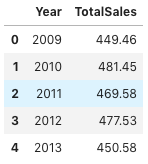
\includegraphics{ex1.png}
\caption{alt text}
\end{figure}

\hypertarget{ux3bbux3cdux3c3ux3b7}{%
\paragraph{Λύση}\label{ux3bbux3cdux3c3ux3b7}}

\begin{verbatim}
SELECT strftime('%Y', invoiceDate) As Year,SUM(Total) As TotalSales 
FROM invoices 
GROUP BY strftime('%Y', invoiceDate)

pd.read_sql_query("SELECT strftime('%Y', invoiceDate) As Year ,SUM(Total) As TotalSales FROM invoices GROUP BY strftime('%Y', invoiceDate)",conn)
\end{verbatim}

    \hypertarget{ux3acux3c3ux3baux3b7ux3c3ux3b7}{%
\subsubsection{Άσκηση}\label{ux3acux3c3ux3baux3b7ux3c3ux3b7}}

Να βρεθούν τα 20 τραγούδια με τις περισσότερες πωλήσεις (και πόσες ήταν
αυτές)

\hypertarget{ux3bbux3cdux3c3ux3b7}{%
\paragraph{Λύση}\label{ux3bbux3cdux3c3ux3b7}}

\begin{verbatim}
SELECT tracks.Name, COUNT(*)
FROM invoice_items
INNER JOIN tracks ON tracks.trackId = invoice_items.trackId
GROUP BY invoice_items.trackId
ORDEF BY count(*) DESC
LIMIT 20

pd.read_sql_query("SELECT tracks.Name, COUNT(*) FROM invoice_items INNER JOIN tracks ON tracks.trackId = invoice_items.trackId GROUP BY invoice_items.trackId ORDER BY count(*) DESC LIMIT 20",conn)
\end{verbatim}

    \hypertarget{if---else}{%
\subsubsection{IF - ELSE}\label{if---else}}

\begin{verbatim}
CASE case_expression
     WHEN when_expression_1 THEN result_1
     WHEN when_expression_2 THEN result_2
     ...
     [ ELSE result_else ] 
END
\end{verbatim}

\begin{verbatim}
SELECT CASE 
        WHEN strftime('%m', invoiceDate) = '01' THEN 'January' 
        WHEN strftime('%m', invoiceDate) = '02' THEN 'February' 
        ELSE '...' 
       END AS Month, 
       invoiceDate 
FROM invoices
\end{verbatim}

    \begin{Verbatim}[commandchars=\\\{\}]
{\color{incolor}In [{\color{incolor}41}]:} \PY{n}{pd}\PY{o}{.}\PY{n}{read\PYZus{}sql\PYZus{}query}\PY{p}{(}\PY{l+s+s2}{\PYZdq{}}\PY{l+s+s2}{SELECT CASE WHEN strftime(}\PY{l+s+s2}{\PYZsq{}}\PY{l+s+s2}{\PYZpc{}}\PY{l+s+s2}{m}\PY{l+s+s2}{\PYZsq{}}\PY{l+s+s2}{, invoiceDate) = }\PY{l+s+s2}{\PYZsq{}}\PY{l+s+s2}{01}\PY{l+s+s2}{\PYZsq{}}\PY{l+s+s2}{ THEN }\PY{l+s+s2}{\PYZsq{}}\PY{l+s+s2}{January}\PY{l+s+s2}{\PYZsq{}}\PY{l+s+s2}{ WHEN strftime(}\PY{l+s+s2}{\PYZsq{}}\PY{l+s+s2}{\PYZpc{}}\PY{l+s+s2}{m}\PY{l+s+s2}{\PYZsq{}}\PY{l+s+s2}{, invoiceDate) = }\PY{l+s+s2}{\PYZsq{}}\PY{l+s+s2}{02}\PY{l+s+s2}{\PYZsq{}}\PY{l+s+s2}{ THEN }\PY{l+s+s2}{\PYZsq{}}\PY{l+s+s2}{February}\PY{l+s+s2}{\PYZsq{}}\PY{l+s+s2}{ ELSE }\PY{l+s+s2}{\PYZsq{}}\PY{l+s+s2}{...}\PY{l+s+s2}{\PYZsq{}}\PY{l+s+s2}{ END AS Month, invoiceDate FROM invoices}\PY{l+s+s2}{\PYZdq{}}\PY{p}{,}\PY{n}{conn}\PY{p}{)}
\end{Verbatim}


\begin{Verbatim}[commandchars=\\\{\}]
{\color{outcolor}Out[{\color{outcolor}41}]:}         Month          InvoiceDate
         0     January  2009-01-01 00:00:00
         1     January  2009-01-02 00:00:00
         2     January  2009-01-03 00:00:00
         3     January  2009-01-06 00:00:00
         4     January  2009-01-11 00:00:00
         5     January  2009-01-19 00:00:00
         6    February  2009-02-01 00:00:00
         7    February  2009-02-01 00:00:00
         8    February  2009-02-02 00:00:00
         9    February  2009-02-03 00:00:00
         10   February  2009-02-06 00:00:00
         11   February  2009-02-11 00:00:00
         12   February  2009-02-19 00:00:00
         13        {\ldots}  2009-03-04 00:00:00
         14        {\ldots}  2009-03-04 00:00:00
         15        {\ldots}  2009-03-05 00:00:00
         16        {\ldots}  2009-03-06 00:00:00
         17        {\ldots}  2009-03-09 00:00:00
         18        {\ldots}  2009-03-14 00:00:00
         19        {\ldots}  2009-03-22 00:00:00
         20        {\ldots}  2009-04-04 00:00:00
         21        {\ldots}  2009-04-04 00:00:00
         22        {\ldots}  2009-04-05 00:00:00
         23        {\ldots}  2009-04-06 00:00:00
         24        {\ldots}  2009-04-09 00:00:00
         25        {\ldots}  2009-04-14 00:00:00
         26        {\ldots}  2009-04-22 00:00:00
         27        {\ldots}  2009-05-05 00:00:00
         28        {\ldots}  2009-05-05 00:00:00
         29        {\ldots}  2009-05-06 00:00:00
         ..        {\ldots}                  {\ldots}
         382       {\ldots}  2013-08-12 00:00:00
         383       {\ldots}  2013-08-20 00:00:00
         384       {\ldots}  2013-09-02 00:00:00
         385       {\ldots}  2013-09-02 00:00:00
         386       {\ldots}  2013-09-03 00:00:00
         387       {\ldots}  2013-09-04 00:00:00
         388       {\ldots}  2013-09-07 00:00:00
         389       {\ldots}  2013-09-12 00:00:00
         390       {\ldots}  2013-09-20 00:00:00
         391       {\ldots}  2013-10-03 00:00:00
         392       {\ldots}  2013-10-03 00:00:00
         393       {\ldots}  2013-10-04 00:00:00
         394       {\ldots}  2013-10-05 00:00:00
         395       {\ldots}  2013-10-08 00:00:00
         396       {\ldots}  2013-10-13 00:00:00
         397       {\ldots}  2013-10-21 00:00:00
         398       {\ldots}  2013-11-03 00:00:00
         399       {\ldots}  2013-11-03 00:00:00
         400       {\ldots}  2013-11-04 00:00:00
         401       {\ldots}  2013-11-05 00:00:00
         402       {\ldots}  2013-11-08 00:00:00
         403       {\ldots}  2013-11-13 00:00:00
         404       {\ldots}  2013-11-21 00:00:00
         405       {\ldots}  2013-12-04 00:00:00
         406       {\ldots}  2013-12-04 00:00:00
         407       {\ldots}  2013-12-05 00:00:00
         408       {\ldots}  2013-12-06 00:00:00
         409       {\ldots}  2013-12-09 00:00:00
         410       {\ldots}  2013-12-14 00:00:00
         411       {\ldots}  2013-12-22 00:00:00
         
         [412 rows x 2 columns]
\end{Verbatim}
            
    \begin{verbatim}
SELECT SUM(CASE 
            WHEN strftime('%m', invoiceDate) = '01' THEN 1 
            ELSE 0 
           END) AS January, 
        SUM(CASE 
            WHEN strftime('%m', invoiceDate) = '02' THEN 1 
            ELSE 0 
        END) AS February
FROM invoices
\end{verbatim}

    \begin{Verbatim}[commandchars=\\\{\}]
{\color{incolor}In [{\color{incolor}42}]:} \PY{n}{pd}\PY{o}{.}\PY{n}{read\PYZus{}sql\PYZus{}query}\PY{p}{(}\PY{l+s+s2}{\PYZdq{}}\PY{l+s+s2}{SELECT SUM(CASE WHEN strftime(}\PY{l+s+s2}{\PYZsq{}}\PY{l+s+s2}{\PYZpc{}}\PY{l+s+s2}{m}\PY{l+s+s2}{\PYZsq{}}\PY{l+s+s2}{, invoiceDate) = }\PY{l+s+s2}{\PYZsq{}}\PY{l+s+s2}{01}\PY{l+s+s2}{\PYZsq{}}\PY{l+s+s2}{ THEN 1 ELSE 0 END) AS January, SUM(CASE WHEN strftime(}\PY{l+s+s2}{\PYZsq{}}\PY{l+s+s2}{\PYZpc{}}\PY{l+s+s2}{m}\PY{l+s+s2}{\PYZsq{}}\PY{l+s+s2}{, invoiceDate) = }\PY{l+s+s2}{\PYZsq{}}\PY{l+s+s2}{02}\PY{l+s+s2}{\PYZsq{}}\PY{l+s+s2}{ THEN 1 ELSE 0 END) AS February FROM invoices}\PY{l+s+s2}{\PYZdq{}}\PY{p}{,}\PY{n}{conn}\PY{p}{)}
\end{Verbatim}


\begin{Verbatim}[commandchars=\\\{\}]
{\color{outcolor}Out[{\color{outcolor}42}]:}    January  February
         0       34        33
\end{Verbatim}
            

    % Add a bibliography block to the postdoc
    
    
    
    \end{document}
